%\newpage
%\section{Заполнение шаблона}
%\begin{itemize}
	%\item Изменить \textbf{config.tex}: имя студента, название предмета и пр. %параметры указаны именно там
	%\item Заполнить \textbf{content.tex} - файл, который будет содержать весь %текст отчёта, от вступления до заключения.
	%\item Добавить используемую литературу (если есть) в \textbf{refs.bib}. Для %удобного поиска источников можно воспользоваться Google Books. Использованные %источники можно указывать с помощью команды \textbf{\\cite\{name\_of\_ref\}}
%\end{itemize}
%Далее представлены различные примеры.

\section{Цель работы}\label{sec:purpose}

Изучение явления затухания люминесценции, понятий квантового выхода и времени жизни на примере эрбиевых лазерных стёкол.

\section{Задачи, решаемые в лабораторной работе}\label{sec:tasks}
\begin{enumerate}
	\item Изучение методик:
		\begin{itemize}
			\item[--] Измерения кинетики затухания люминесценции.
			\item[--] Расчета среднего времени жизни люминесценции
			\item[--] Расчета радиационного времени жизни по методу Фюхтенбауэра – Ланденбурга
			\item[--] Определения квантового выхода люминесценции
		\end{itemize}
	\item Ознакомление с понятием о передачи возбуждений между локальными
			оптическими центрами, основными представлениями о механизмах
			ответственных за передачу
	\item Изучить экспериментальные проявления передачи возбуждений(сенсибилизация, тушение)
	\item Для концентрационного ряда эрбиевых стёкол:
		\begin{itemize}
			\item[--] Измерить на экспериментальной установке время затухания люминесценции
			\item[--] Провести расчет радиационного времени жизни
			\item[--] Расчета радиационного времени жизни по методу Фюхтенбауэра – Ланденбурга
			\item[--] Определить квантовый выход люминесценции
		\end{itemize}
\end{enumerate}

\section{Объект исследования}\label{sec:object}

Лазерные стекла, активированные ионами эрбия
%\section{Теоретическая информация}\label{sec:теоретическая-информация}

%Было использовано методическое указание по выполнению лабораторного практикума по основам фотоники.
%Исследование кинетических свойств фотохромных стекол~\cite{conlan1983massive}.

\section{Рабочие формулы и исходные данные}\label{sec:initial_data}

%\begin{equation}
%a= \begin{cases}
% 3x + 5y + z, \mbox{если хорошо} \\
% 7x - 2y + 4z, \mbox{если плохо}\\
% -6x + 3y + 2z, \mbox{если совсем плохо}
%\end{cases}
%\label{eq:F10}
%\end{equation}

\begin{equation}
\tau{_{rad}^{-1}} = 8 \cdot \pi \cdot c
					\cdot n^2 \cdot \tilde{\nu}^2 \cdot \frac{8}{7}
					\cdot \int \sigma_{abs}(\nu)d\nu
\label{eq:F1}
\end{equation}
где $c$ – скорость света, $n$ – показатель преломления стекла,
$\tilde{\nu}$ – средняя частота полосы, $\int \sigma_{abs}(\nu)d\nu$
– интегральное сечение поглощение основного
резонансного перехода
${}^4$$I_{15/2}\rightarrow{}^4$$I_{13/2}$

%\rightarrow\sideset{^4}{_{13/2}}I
\begin{equation}
q = (\tau_{exp}/\tau_{rad}) \cdot 100\%,
\label{eq:F2}
\end{equation}
где $\tau_{exp}$ – экспериментально определенное время
жизни люминесценции перехода
${}^4$$I_{15/2}\rightarrow{}^4$$I_{13/2}$,
$\tau_{rad}$ – радиационное время жизни люминесценции перехода
${}^4$$I_{15/2}\rightarrow{}^4$$I_{13/2}$.

\section{Оборудования и принадлежности}\label{sec:stuff}
\subsection{Схема установки}\label{subsec:schemes}
\begin{figure}[H]
        \centering
        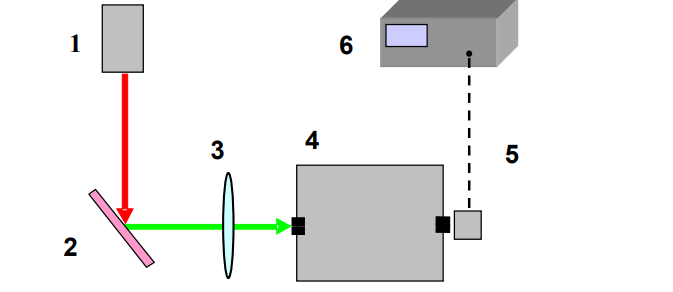
\includegraphics[width=0.7\columnwidth]{figures/Scheme}%[width=]
        \caption{Схема установки для определения кинетики затухания
люминесценции. Цифрами на схеме обозначены: (1) – импульсный лазер; (2)
– образец; (3) – короткофокусный объектив; (4) – монохроматор; (5) –
InGaAs-приемник (6) –осциллограф}
		\label{fig:Scheme}
\end{figure}
\section{Результаты эксперимента}\label{sec:results}

Построили зависимость нормированной интенсивности
люминесценции от времени для каждого из образцов.[\ref{fig:someFigure1}] - [\ref{fig:someFigure6}]
По площади графиков [\ref{fig:someFigure1}] - [\ref{fig:someFigure6}] мы определили время затухания люминесценции для каждого из образцов.

Построили зависимость значений времени жизни люминесценции
от концентрации ионов эрбия [\ref{fig:Concentration}]

По формуле [\ref{eq:F1}] мы определили значение радиационного времени
жизни люминесценции.
Используя параметры образцов и формулу [\ref{eq:F2}] определили квантовый выход люминесценции для всех образцов.
Исходные данные, которые использовались для расчетов приведены в таблице \ref{tab:info}.
Полученные значения занесены в таблицу \ref{tab:times}.

По полученным результатам можно сказать, что при увеличении концентрации ионов-активаторов в стекле время затухания люминесценции сокращается.
Однако неточность алгоритма Левенберга — Марквардта (некоторые переменные были заданы вручную, чтобы экспонатна стремилась к 0) привело к неточным измерениям времени жизни,
так как явной зависимости времени затухания люминесценции от концентрации ионов-активаторов не наблюдается.

Построили зависимость квантового выхода люминесценции от концентрации ионов эрбия. [\ref{fig:someFigure0}]

% Please add the following required packages to your document preamble:
% \usepackage{multirow}
% \usepackage{graphicx}
\begin{table}[]
\centering
\caption{Результаты вычислений параметров исследуемых образцов}
\label{tab:times}
\resizebox{\textwidth}{!}{%
\begin{tabular}{|c|c|c|c|c|}
\hline
\multirow{2}{*}{Номер серии} & \multirow{2}{*}{Номер образца} & Экспериментальное время       & Радиационное время          & Квантовый выход   \\
                             &                                & затухания   люминесценции, мс & затухания люминесценции, мс & люминесценции, \% \\ \hline
\multirow{3}{*}{1}           & 340                            & 6,29                          & \multirow{3}{*}{8,616}      & 73,00             \\ \cline{2-3} \cline{5-5}
                             & 342                            & 5,65                          &                             & 65,58             \\ \cline{2-3} \cline{5-5}
                             & 343                            & 1,78                          &                             & 20,66             \\ \hline
\multirow{4}{*}{2}           & 344                            & 9,88                          & \multirow{4}{*}{15,837}     & 62,39             \\ \cline{2-3} \cline{5-5}
                             & 345                            & 10,28                         &                             & 64,91             \\ \cline{2-3} \cline{5-5}
                             & 346                            & 9,62                          &                             & 60,74             \\ \cline{2-3} \cline{5-5}
                             & 347                            & 9,61                          &                             & 60,68             \\ \hline
\end{tabular}%
}
\end{table}

% Please add the following required packages to your document preamble:
% \usepackage{graphicx}
\begin{table}[H]
\centering
\caption{Исходные данные для используемых образцов}
\label{tab:info}
\resizebox{\textwidth}{!}{%
\begin{tabular}{|c|c|c|c|c|}
\hline
Номер серии & Номер образца & \begin{tabular}[c]{@{}c@{}}Концентрация ионов\\     эрбия, 1020 см-1\end{tabular} & \begin{tabular}[c]{@{}c@{}}Показатель\\  преломления\end{tabular} & \begin{tabular}[c]{@{}c@{}}Интегральное сечение \\ поглощения, \\    10–18 см\end{tabular} \\ \hline
            & 340           & 0,50                                                                              &                                                                   &                                                                                            \\ \cline{2-3}
1           & 342           & 0,15                                                                              & 1,554                                                             & 1,340                                                                                      \\ \cline{2-3}
            & 343           & 8,50                                                                              &                                                                   &                                                                                            \\ \hline
            & 344           & 0,26                                                                              &                                                                   &                                                                                            \\ \cline{2-3}
2           & 345           & 0,56                                                                              & 1,520                                                             & 0,762                                                                                      \\ \cline{2-3}
            & 346           & 1,12                                                                              &                                                                   &                                                                                            \\ \cline{2-3}
            & 347           & 1,12                                                                              &                                                                   &                                                                                            \\ \hline
\end{tabular}%
}
\end{table}

\section{Графики}\label{sec:graphics}
 Оптимизируем функции с помощью алгоритма Левенберга — Марквардта\cite{levenberg1944method}
\begin{figure}[H]
	\centering
	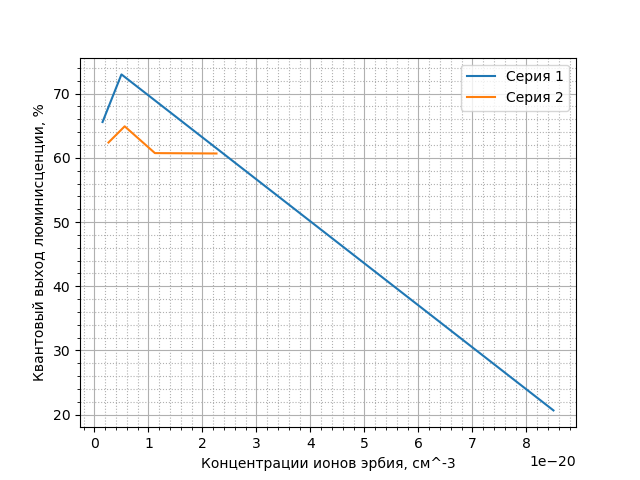
\includegraphics[width=2.8in]{figures/ContcentrationTheory}
	\caption{зависимость квантового выхода люминесценции от
концентрации иона активатора}
	\label{fig:someFigure0}
\end{figure}

\begin{figure}[H]
	\centering
	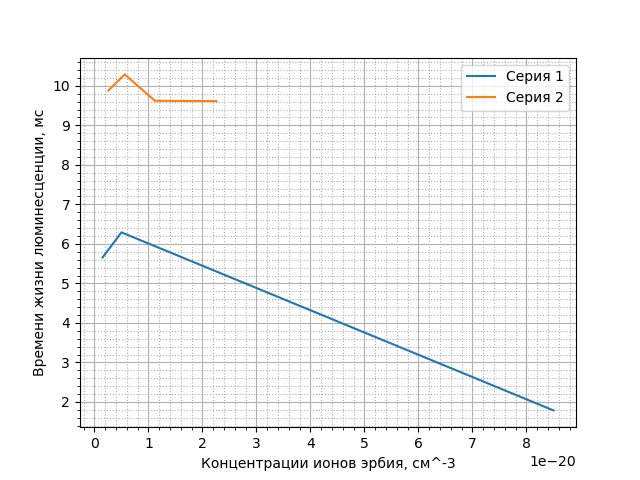
\includegraphics[width=2.8in]{figures/Contcentration}
	\caption{Зависимость значений времени жизни люминесценции
от концентрации ионов эрбия}
	\label{fig:Concentration}
\end{figure}

\begin{figure}[H]
\centering

\subfigure{
\begin{minipage}[t]{0.5\linewidth}
\centering
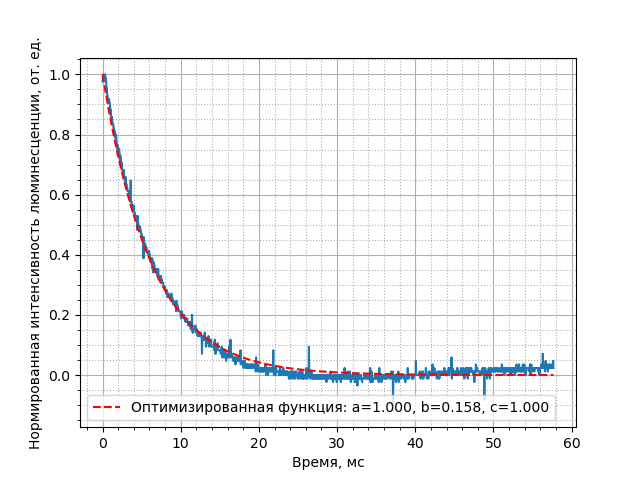
\includegraphics[width=2.8in]{figures/I_340}
\caption{Зависимость изменения интенсивности люминесценции
во времени для образца №1}
\label{fig:someFigure1}
\end{minipage}%
}%
\subfigure{
\begin{minipage}[t]{0.5\linewidth}
\centering
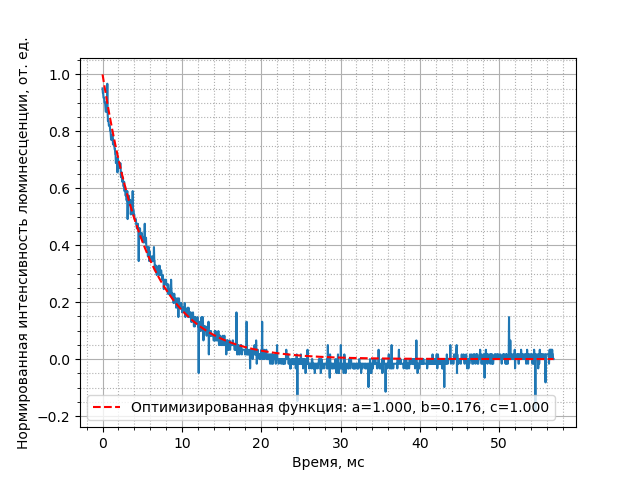
\includegraphics[width=3in]{figures/I_342}
\caption{Зависимость изменения интенсивности люминесценции
во времени для образца №2}
	\label{fig:someFigure2}
\end{minipage}%
}%

\subfigure{
\begin{minipage}[t]{0.5\linewidth}
\centering
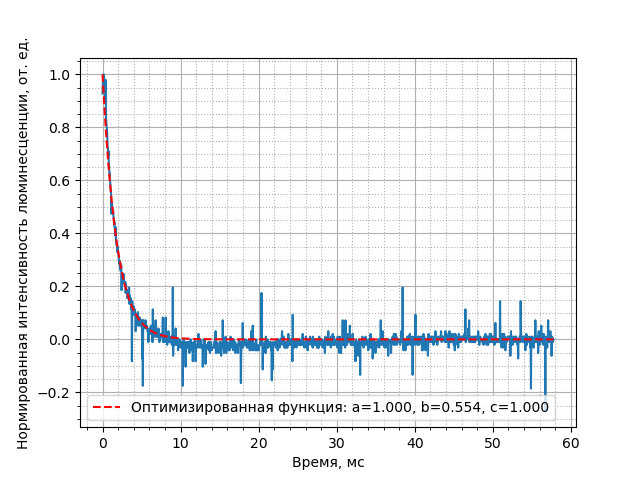
\includegraphics[width=2.8in]{figures/I_343}
\caption{Зависимость изменения интенсивности люминесценции
во времени для образца №3}
	\label{fig:someFigure3}
\end{minipage}
}%
\subfigure{
\begin{minipage}[t]{0.5\linewidth}
\centering
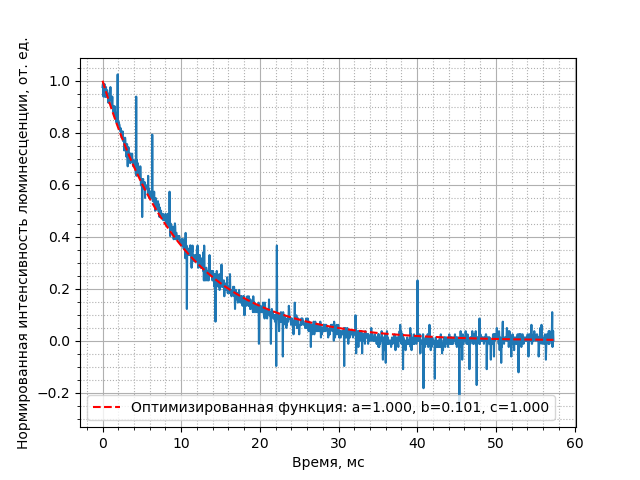
\includegraphics[width=3in]{figures/I_344}
\caption{Зависимость изменения интенсивности люминесценции
во времени для образца №4}
	\label{fig:someFigure4}
\end{minipage}
}%
\centering

\end{figure}
\begin{figure}[H]
\centering
	\subfigure{
		\begin{minipage}[t]{0.5\linewidth}
		\centering
		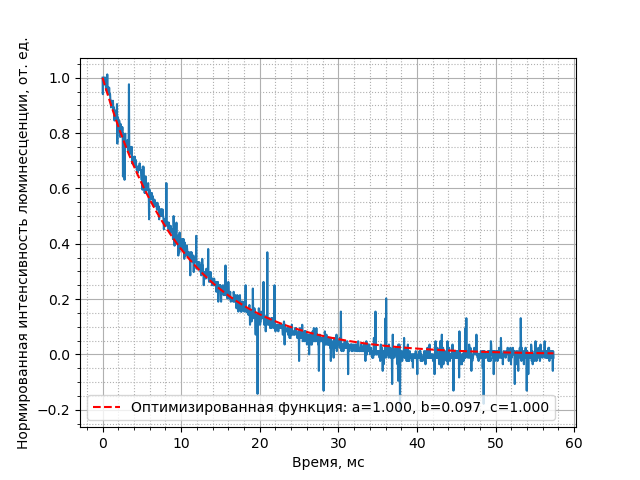
\includegraphics[width=3in]{figures/I_345}
		\caption{Зависимость изменения интенсивности люминесценции
		во времени для образца №5}
			\label{fig:someFigure5}
		\end{minipage}
	}%
	\subfigure{
		\begin{minipage}[t]{0.5\linewidth}
		\centering
		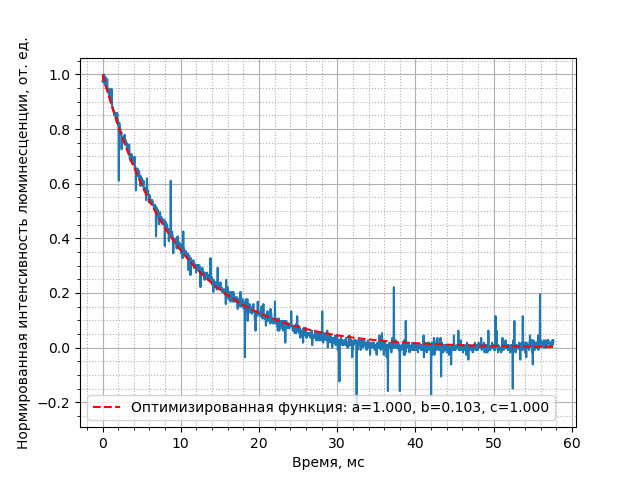
\includegraphics[width=3in]{figures/I_346}
		\caption{Зависимость изменения интенсивности люминесценции
		во времени для образца №6}
			\label{fig:someFigure6}
		\end{minipage}
	}%
\centering

\end{figure}

\begin{figure}[H]
	\centering
	\subfigure{
		\begin{minipage}[t]{0.5\linewidth}
		\centering
		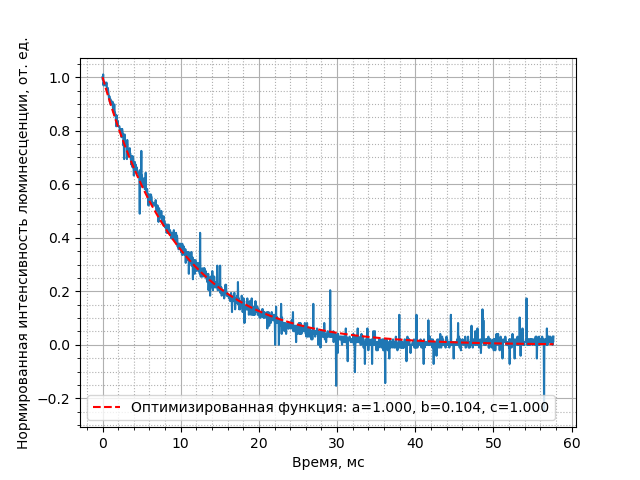
\includegraphics[width=3in]{figures/I_347}
		\caption{Зависимость изменения интенсивности люминесценции
		во времени для образца №7}
			\label{fig:someFigure7}
		\end{minipage}
	}%
	\centering
\end{figure}

\section{Выводы и анализы результатов}\label{sec:conclution}
В процессе выполнения лабораторной работы на основе методического пособия\cite{AseevMetoda}, были изучены явления затухания люминесценции,
понятия квантового выхода и времени жизни люминесценции на примере эрбиевых лазерных стёкол.
Были зарегистрированы кривые затухания люминесценции для двух серий образцов с определёнными показателями преломления для каждой из серий.
Исследована зависимость кинетики затухания люминесценции от концентрации ионов-активаторов,
рассчитаны радиационные времена затухания люминесценции для двух серий образцов, вычислен квантовый выход люминесценции.

В результате лабораторной работы было зарегистрировано,
что образцам с более высокой концентрацией ионов-активаторов соответствуют менее длительные времена затухания.
При относительно небольшой концентрации эта зависимость не наблюдается так ярко.
Аналогичная зависимость квантового выхода люминесценции образцов от концентрации ионов эрбия.

